\documentclass{article} % For LaTeX2e
\usepackage{nips14submit_e,times}
\usepackage{hyperref}
\usepackage{url}
\usepackage[leqno, fleqn]{amsmath}
\usepackage{amssymb}
\usepackage{qtree}
\usepackage[numbers]{natbib}
\usepackage{graphicx}
\usepackage{booktabs}
\usepackage{colortbl}
\usepackage{caption}
\usepackage{subcaption}
\usepackage{xcolor}



\definecolor{mylinkcolor}{rgb}{0,0,0} % black
\hypersetup{colorlinks, linkcolor=mylinkcolor, urlcolor=mylinkcolor, citecolor=mylinkcolor}

\newcommand{\nateq}{\equiv}
\newcommand{\natind}{\mathbin{\#}}
%\newcommand{\natneg}{\raisebox{2px}{\tiny\thinspace$\wedge$\thinspace}}
\newcommand{\natneg}{\mathbin{^{\wedge}}}
\newcommand{\natfor}{\sqsubset}
\newcommand{\natrev}{\sqsupset}
\newcommand{\natalt}{\mathbin{|}}
\newcommand{\natcov}{\mathbin{\smallsmile}}

\newcommand{\plneg}{\mathop{\textit{not}}}
\newcommand{\pland}{\mathbin{\textit{and}}}
\newcommand{\plor}{\mathbin{\textit{or}}}



% Strikeout
\newlength{\howlong}\newcommand{\strikeout}[1]{\settowidth{\howlong}{#1}#1\unitlength0.5ex%
\begin{picture}(0,0)\put(0,1){\line(-1,0){\howlong\divide\unitlength}}\end{picture}}

\newcommand{\True}{\texttt{T}}
\newcommand{\False}{\texttt{F}}
\usepackage{stmaryrd}
\newcommand{\sem}[1]{\ensuremath{\llbracket#1\rrbracket}}


\renewcommand{\bibsection}{\subsubsection*{References}}

\usepackage{gb4e}

\def\ii#1{\textit{#1}}

\newcommand{\mynote}[1]{{\color{red}\framebox{\begin{tabular}{p{0.9\textwidth}}\footnotesize#1 \end{tabular}}}}


\title{Recursive Neural Networks for Learning Logical Semantics}

\author{
Samuel R.\ Bowman$^{\ast\dag}$ \\
\texttt{sbowman@stanford.edu} \\[2ex]
$^{\ast}$Stanford Linguistics \\
\And
Christopher Potts$^{\ast}$\\
\texttt{cgpotts@stanford.edu} \\[2ex]
$^{\dag}$Stanford NLP Group
\And
Christopher D.\ Manning$^{\ast\dag\ddag}$\\
\texttt{manning@stanford.edu}\\[2ex]
$^{\ddag}$Stanford Computer Science
}

% \author{
% Samuel R.\ Bowman \\
% NLP Group, Dept.\ of Linguistics\\
% Stanford University\\
% Stanford, CA 94305-2150 \\
% \texttt{sbowman@stanford.edu}
%  \And
%  Christopher Potts \\
% Dept.\ of Linguistics\\
% Stanford University\\
% Stanford, CA 94305-2150 \\
% \texttt{cgpotts@stanford.edu}
%  \And
% Christopher D.\ Manning \\
% NLP Group,  Depts.\ of Computer Science and Linguistics\\
% Stanford University\\
% Stanford, CA 94305-2150 \\
% \texttt{manning@stanford.edu}
% }

\newcommand{\fix}{\marginpar{FIX}}
\newcommand{\new}{\marginpar{NEW}}

\nipsfinalcopy % Uncomment for camera-ready version

\begin{document}
\maketitle

  Supervised recursive neural network models (RNNs) for sentence
  meaning have been successful in an array of sophisticated language
  tasks, but it remains an open question whether they can learn
  compositional semantic grammars that support logical deduction.  We
  address this question directly by for the first time evaluating
  whether each of two classes of neural model --- plain RNNs and
  recursive neural tensor networks (RNTNs) --- can correctly learn
  relationships such as entailment and contradiction between pairs of
  sentences, where we have generated controlled data sets of sentences
  from a logical grammar.  Our first experiment evaluates whether
  these models can learn the basic algebra of logical relations
  involved. Our second and third experiments extend this evaluation to
  complex recursive structures and sentences involving quantification.
  We find that the plain RNN achieves only mixed results on all three
  experiments, whereas the stronger RNTN model generalizes well in
  every setting and appears capable of learning suitable
  representations for natural language logical inference.
  
  \section{Introduction}\label{sec:intro}

Supervised recursive neural network models (RNNs) for sentence meaning
have been successful in an array of sophisticated language tasks,
including sentiment analysis \cite{socher2011semi,socher2013acl1},
image description \cite{sochergrounded}, and paraphrase detection
\cite{Socher-etal:2011:Paraphrase}. These results are encouraging for
the ability of these models to learn compositional semantic grammars,
but it remains an open question whether they can achieve the same
results as grammars based in logical forms
\cite{Warren:Pereira:1982,Zelle:Mooney:1996,ZetCol:2005,LiangJordan:2013}
when it comes to the core semantic concepts of quantification,
entailment, and contradiction needed to identify the relationships
between sentences like \ii{every animal walks}, \ii{every turtle
  moves}, and \ii{most reptiles don't move}. To date, experimental
investigations of these concepts using distributed representations
have been largely confined to short phrases
\cite{Mitchell:Lapata:2010,Grefenstette-etal:2011,baroni2012entailment,kalchbrenner2014convolutional}.
For robust natural language understanding, it is essential to model
these phenomena in their full generality on complex linguistic
structures.

We address this question in the context of \ii{natural language
  inference} (also known as \ii{recognizing textual entailment};
\cite{dagan2006pascal}), in which the goal is to determine the core
inferential relationship between two sentences. Much of the
theoretical work on this task (and some successful implemented models
\cite{maccartney2009extended,watanabe2012latent}) involves \ii{natural
  logics}, which are formal systems that define rules of inference
between natural language words, phrases, and sentences without the
need of intermediate representations in an artificial logical
language. Following \cite{bowman2013can}, we use the natural logic
developed by \cite{maccartney2009extended} as our formal model. This
logic defines seven core relations of synonymy, entailment,
contradiction, and mutual consistency, as summarized in
Table~\ref{b-table}, and it provides rules of semantic combination for
projecting these relations from the lexicon up to complex phrases. The
formal properties and inferential strength of this system are now
well-understood \cite{Icard:Moss:2013,Icard:Moss:2013:LILT}.

In our experiments, we use this pre-specified logical grammar to
generate controlled data sets encoding the semantic relationships
between pairs of expressions and evaluate whether each of two classes
of neural model --- plain RNNs and recursive neural tensor networks
(RNTNs, \cite{socher2013acl1}) --- can learn those relationships
correctly. In our first experiment (Section~\ref{sec:join}), we
evaluate the ability of these models to learn the core relational
algebra of natural logic from data. Our second experiment
(Section~\ref{sec:recursion}) extends this evaluation to relations
between complex recursive structures like $(a \plor b)$ and
$\plneg(\plneg a \pland \plneg b)$, and our third experiment
(Section~\ref{sec:quantifiers}) involves relations between quantified
statements like \ii{every reptile walks} and \ii{no turtle moves}.
We find that the plain RNN achieves only mixed results in all three
experiments, whereas the stronger RNTN model generalizes well in every
case, suggesting that it has in fact learned, or at least learned to
simulate, our target logical
concepts. These experiments differentiate the increased power of RNTNs
better than previous work and provide the most convincing
demonstration to date of the ability of neural networks to model
semantic inferences in complex natural language sentences.

\begin{table}[tp]
  \centering
  \setlength{\tabcolsep}{15pt}
  \renewcommand{\arraystretch}{1.1}
  \begin{tabular}{l c l l} 
    \toprule
    Name & Symbol & Set-theoretic definition & Example \\ 
    \midrule
    entailment         & $x \natfor y$   & $x \subset y$ & \ii{turtle, reptile}  \\ 
    reverse entailment & $x \natrev y$   & $x \supset y$ & \ii{reptile, turtle}  \\ 
    equivalence        & $x \nateq y$    & $x = y$       & \ii{couch, sofa} \\ 
    alternation        & $x \natalt y$   & $x \cap y = \emptyset \wedge x \cup y \neq \mathcal{D}$ & \ii{turtle, warthog} \\ 
    negation           & $x \natneg y$   & $x \cap y = \emptyset \wedge x \cup y = \mathcal{D}$    & \ii{able, unable} \\
    cover              & $x \natcov y$   & $x \cap y \neq \emptyset \wedge x \cup y = \mathcal{D}$ & \ii{animal, non-turtle} \\ 
    independence       & $x \natind y$   & (else) & \ii{turtle, pet}\\
    \bottomrule
  \end{tabular}
  \caption{The seven natural logic relations of \cite{maccartney2009extended}. 
    $\mathcal{D}$ is the universe of possible objects of the same type as those being compared, 
    and the relation $\natind$ applies whenever none of the other six do.} %, including when there 
    %is insufficient knowledge to choose a label.}
  \label{b-table}
\end{table}


% Citations to additional past work to be added.\\...\\...\\...\\...\\...


% Deep learning methods in NLP which learn vector representations for words have seen successful uses in recent years on increasingly sophisticated tasks \cite{collobert2011natural, socher2011semi, socher2013acl1, chen2013learning}. Given the still modest performance of semantically rich NLP systems in many domains---question answering and machine translation, for instance---it is worth exploring the degree to which learned vectors can serve as general purpose semantic representations. Much of the work to date analyzing vector representations for words (see \cite{baroni2013frege}) has focused on lexical semantic behaviors---like the similarity between words like \ii{Paris} and \ii{France}. Good similarity functions are valuable for many NLP tasks, but there are real use cases for which it is necessary to know how words relate to one another or to some extrinsic representation, and to model the ways in which word meanings combine to form phrase, sentence, or document meanings. This paper explores the ability of linguistic representations developed using supervised deep learning techniques to support interpretation and reasoning. 

% There are two broad family of tasks that could be used to test the ability of a model to develop general purpose meaning representations. In an interpretation task, sentences are mapped onto some denotation, such as  \ii{true} or \ii{false} for statements, or a factual answer for questions. There has been preliminary work in developing distributed models for interpretation \cite{grefenstette2013towards, rocktaschellow}, but developing a representation of world knowledge that corresponds accurately to the content expressed in language introduces considerable design challenges. I approach the problem by way of an inference task instead. Inferring the truth of one sentence from another does not require any preexisting knowledge representations, but nonetheless requires a precise representation of sentence meaning. I borrow the structure of the task from MacCartney and Manning  \cite{maccartney2009extended}. In it, the model is presented with a pair of sentences, and made to label the logical relation between the sentences as equivalence, entailment, or any of five other classes, as here:

%\begin{quote}
%\begin{enumerate}\small
%\item Many smartphone users avoid high bills overseas by disabling data service.
%\item Not everyone uses their smartphones for email when traveling abroad.
%\end{enumerate} 
%$\Rightarrow$ Entailment
%\end{quote}

%In this paper, we test the ability of recursive models to on three simple tasks, each of which is meant to capture a property that is necessary in representing natural language meaning in the setting of inference. I begin with an overview of MacCartney and Manning's \cite{maccartney2009extended} framework for inference, and of the recursive neural networks that I study. by showing that these models can learn to correctly represent entailment representations between sentences. I then show that these models can capture the meanings of recursive structures accurately up to a sufficient depth. I finally close with a brief demonstration of the ability of these models to reason over short natural language sentences involving quantifiers. 

% \subsection{Natural language inference and natural logic}

% In its simplest form, \ii{natural language inference} (also known as \ii{recognizing textual entailment}, as in \cite{dagan2006pascal}) is the task of determine whether one sentence entails another. Much of the theoretical work on this task (and some successful implemented models \cite{maccartney2009natural, watanabe2012latent}) involve \ii{natural logic}, formal systems that define sound rules of inference from one sentence of natural language to another without the need for intermediate representations in some other logic. The most powerful model that we are aware of for natural logic is due to MacCartney and Manning \cite{maccartney2009extended} and Icard \cite{icard2012inclusion}, and is centered around the definition of a set of seven logical relations which can hold between sentences, shown in Table \ref{b-table}.

% This approach to natural logic can capture much of the complexity of natural language meaning within a well understood framework, and is also fairly straightforward to implement in a machine learning setting since it can be reduced to a seven-way classification problem on sentence pairs. Our goal in this paper is to learn recursive neural network models which are able to mimic key behaviors of this system.

% \begin{table}
% \begin{center}
% \begin{tabular}{|c|c|c|c|} \hline
% name & symbol & set-theoretic definition & example \\ \hline \hline
% entailment & $x \sqsubset y$ & $x \subset y$ & \ii{crow, bird}  \\ \hline
% reverse entailment & $x \sqsupset y$ & $x \supset y$ & \ii{Asian, Thai}  \\ \hline
% equivalence & $x \equiv y$ & $x = y$ & \ii{couch, sofa} \\ \hline
% alteration & $x$ $|$ $y$ & $x \cap y = \emptyset \wedge x \cup y \neq \mathcal{D}$ & \ii{cat, dog} \\ \hline
% negation & $x \natneg y$ & $x \cap y = \emptyset \wedge x \cup y = \mathcal{D}$ & \ii{able, unable} \\ \hline
% cover & $x \smallsmile y$ & $x \cap y \neq \emptyset \wedge x \cup y = \mathcal{D}$ & \ii{animal, non-ape} \\ \hline
% independence & $x$ \# $y$ & (else) & \ii{hungry, hippo}\\ \hline
% \end{tabular}
% \caption{The entailment relations in  $\mathfrak{B}$. $\mathcal{D}$ is the universe of possible objects of the same type as those being compared, and the relation \# applies whenever none of the other six do, including when there is insufficient knowledge to choose a label.}
% \label{b-table}
% \end{center}
% \end{table}

% The goal of each of the three experiments that we propose is to learn classifiers that are able to classify pairs of statements from some highly constrained language into these seven classes. It should be noted that this is not a balanced classification problem. If arbitrary pairs of statements are chosen for comparison in almost any domain of natural language, the minimally informative \# relation will apply between them. % TODO: How much should we say about this?


% The natural logic engine at the core of MacCartney and Manning's system requires a complex set of linguistic knowledge, much of which takes the form of what he calls projectivity signatures. These signatures are tables showing the entailment relation that must hold between two strings that differ in a given way (such as the substitution of the argument of some quantifier), and are explicitly provided to the model
%for dozens of different cases of insertion, deletion and substitution of different types of lexical item. For example in judging the inference \ii{no animals bark $|$ some dogs bark} it would first used stored knowledge to compute the relations introduced by each of the two differences between the sentences. Here, the substitution of \ii{no} for \ii{some}  yields $\natneg$ and the substitution of \ii{dogs} for \ii{animals} yields $\sqsupset$. It would then use an additional store of knowledge about relations to resolve the resulting series of relations into one ($|$) that expresses the relation between the two sentences being compared:
%\begin{quote}

%1. \ii{no animals bark $\natneg$ \textbf{some} animals bark}\\
%2. \ii{some animals bark $\sqsupset$ some \textbf{dogs} bark}\\
%3. \ii{no animals bark $[\natneg\bowtie\thinspace\sqsupset\thinspace = |]$ some dogs bark}

%\end{quote}

% Work to date on inference in neural network models is quite limited.
% \citet{baroni2012entailment} have achieved limited success in building a classifier to judge entailments between one- and two-word phrases (including some with quantifiers), though their vector representations were crucially based on distributional statistics and were not  learned for the task.
% In another line of research, \citet{garrette2013formal} propose a way to improve standard discrete NLI with vector representations. They propose a deterministic inference engine (similar to MacCartney's) which is augmented by a probabilistic component that evaluates individual lexical substitution steps in the derivation using vector representations, though again these representations are not learned, and no evaluations of this system have been published to date.
% \label{sec2}


\section{Recursive neural network models} \label{methods}

We study neural models that adhere to the linguistic \ii{principle of
 compositionality}, which says that the meanings for complex
expressions are derived from the meanings of their constituent parts
via specific composition functions \cite{Partee84,Janssen97}. In our
distributed setting, word meanings are vectors of length $n$. The
composition function maps pairs of them to single vectors of length $n$, 
which can then be merged again to represent more complex
phrases. Once the entire sentence-level representation has been
derived, it serves as a fixed-length input for some subsequent function.

We use the model architecture proposed in \cite{bowman2013can} and
depicted in Figure~\ref{sample-figure}. The two phrases being compared
are built up separately on each side of the tree, using the same
composition function, until they have each been reduced to single
vectors. The resulting vectors are fed into a separate comparison
layer that is meant to generate a feature vector capturing the
relation between the two phrases. The output of this layer is then
given to a softmax classifier, which in turn produces a hypothesized
distribution over the seven relations represented in Table~\ref{b-table}.


For a composition layer, we evaluate models with both the plain neural
network layer function \eqref{rnn} and the RNTN layer function
\eqref{rntn} proposed in \citet{chen2013learning}. A sigmoid
nonlinearity (element-wise $\tanh$) is applied to the output of either
layer function, following \cite{socher2013acl1}.
%
\begin{gather} \label{rnn}
\vec{y}_{\textit{RNN}} = f(\mathbf{M} [\vec{x}^{(l)}; \vec{x}^{(r)}] + \vec{b}) \\ % TODO: Add column vectors?
\label{rntn}
\vec{y}_{\textit{RNTN}} = f(\vec{x}^{(l)T} \mathbf{T}^{[1 \ldots n]} \vec{x}^{(r)} + \mathbf{M} [\vec{x}^{(l)}; \vec{x}^{(r)}] + \vec{b})
\end{gather} 
%
Here, $\vec{x}^{(l)}$ and $\vec{x}^{(r)}$ are the column vector
representations for the left and right children of the node, and
$\vec{y}$ is the node's output.  The RNN concatenates them, multiplies
them by an $n \times 2n$ matrix of learned weights, and applies the
element-wise non-linearity to the resulting vector. The RNTN has the
same basic structure, but with the addition of a learned third-order
tensor $\mathbf{T}$, dimension $n \times n \times n$, modeling
multiplicative interactions between the child vectors. Both models
include a bias vector~$\vec{b}$.

The comparison layer uses the same kind of function template as the
composition layers (either an NN layer or an NTN layer) with
independently learned parameters and a separate nonlinearity function.
Rather than use a $\tanh$ nonlinearity here, we follow \cite{bowman2013can} 
in using a rectified linear function. In
particular, we use the leaky rectified linear function
\cite{maasrectifier}: $f(\vec{x})=\max(\vec{x}, 0) +
0.01\min(\vec{x}, 0)$, applied element-wise.

To run the model forward and label a pair of phrases, the structure of
the lower layers of the network is assembled so as to mirror the tree
structures provided for each phrase. The word vectors are then looked
up from the vocabulary matrix $V$ (one of the model parameters), and
the composition and comparison functions are used to pass information
up the tree and into the classifier at the top. For an objective
function, we use the negative log of the probability assigned to the
correct label.

% Removed 'minibatch' -> For two of the experiments, we use minibatches
% of size 1, which doesn't really count.
We train the model using stochastic gradient descent (SGD)
with learning rates computed using AdaGrad \cite{duchi2011adaptive}.
The parameters (including the vocabulary) are initialized randomly 
using a uniform distribution over $[-0.1, 0.1]$.
Because the seven classes are not balanced in general, we report performance
using both accuracy and macroaveraged F1, since the latter emphasizes
 performance on infrequent classes. We compute macroaveraged F1 
as the harmonic mean of mean precision and mean recall, both computed
for all classes for which there is test data, setting precision to 0 
where it is not defined. Source code and generated data will be released
after the review period.

%\begin{figure}[tp]
%  \centering
% % 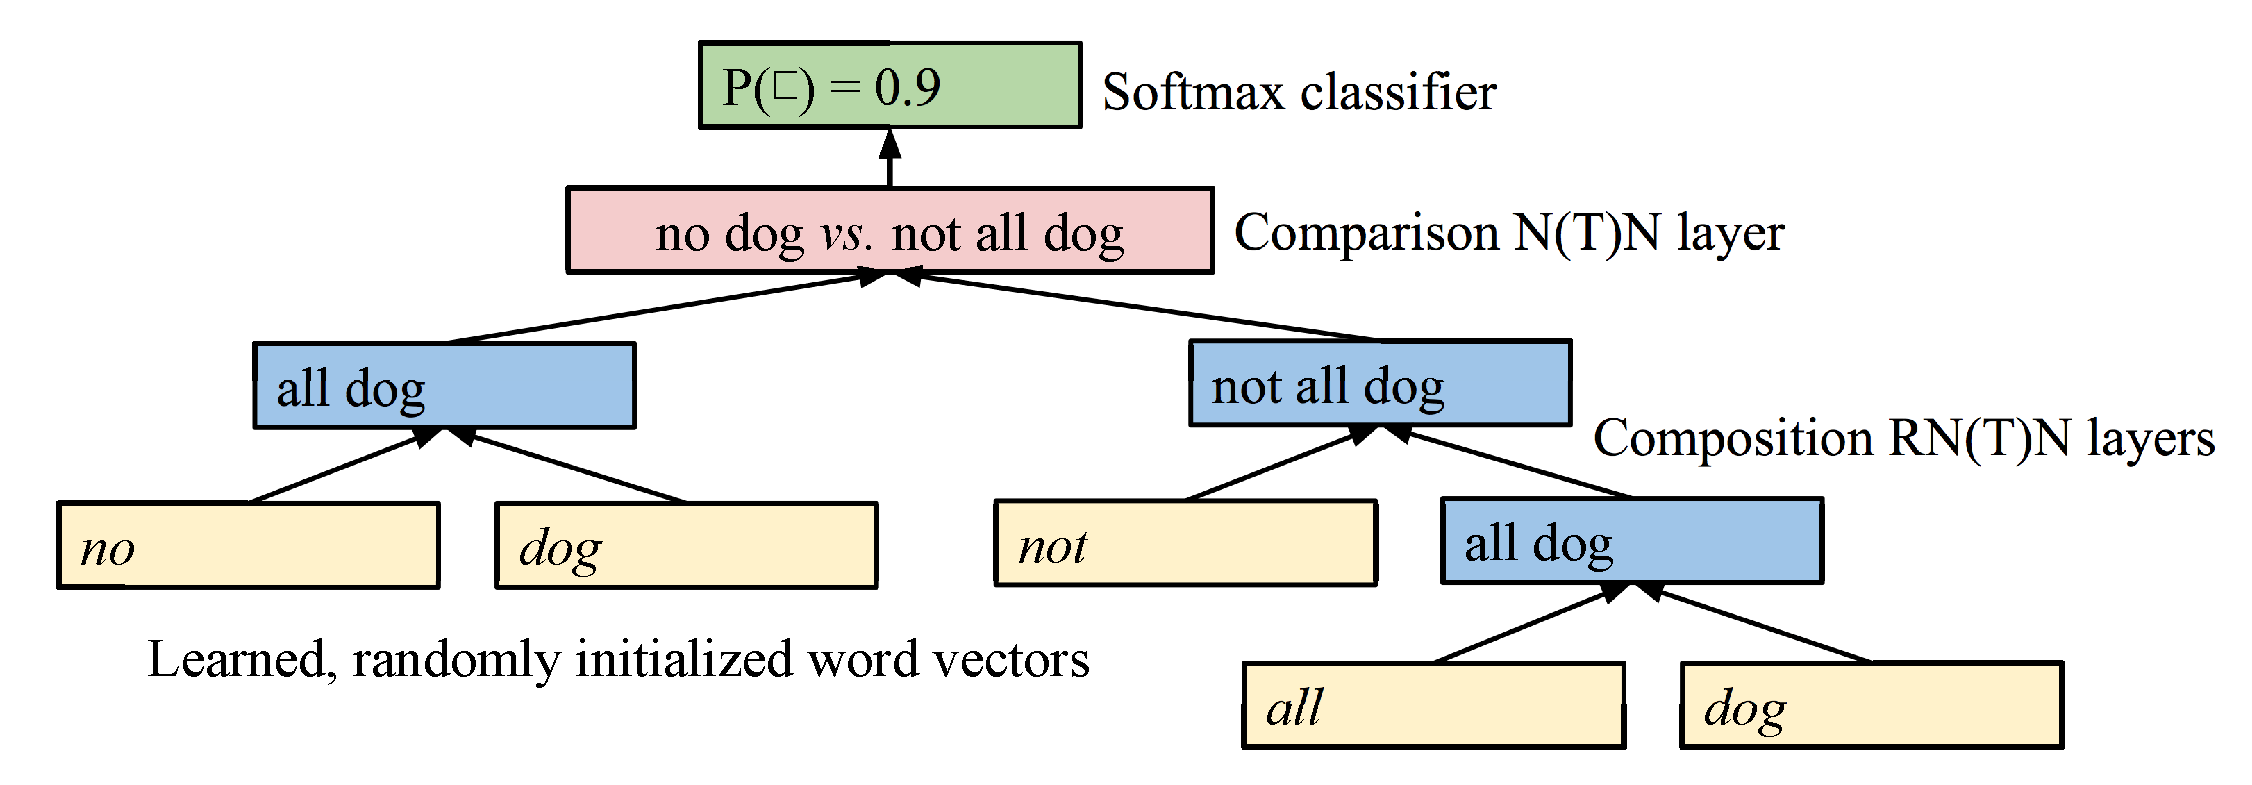
\includegraphics[scale=0.35]{model.eps}
%  \footnotesize

\newcommand{\labeledtreenode}[4][3.5]{\put(#2){\makebox(0,0){{\fcolorbox{black}{#4}{\makebox(#1,0.3){#3}}}}}}

\newcommand{\textlabel}[4][3.5]{\put(#2){\makebox(0,0){{\fcolorbox{white}{white}{\makebox(#1,0.3){#3}}}}}}

\definecolor{lexcolor}{HTML}{F5F7C4}
\definecolor{compositioncolor}{HTML}{BBEBFF}
\definecolor{comparisoncolor}{HTML}{FFC895}
\definecolor{softmaxcolor}{HTML}{A5FF8A}


\setlength{\unitlength}{0.61cm}
\begin{picture}(21,7.5)
  
  \labeledtreenode[2.4]{11.5,7}{$P(\sqsubset) = 0.8$}{softmaxcolor}  
  \put(11.5,5.7){\vector(0,1){1}}  
  \labeledtreenode[7.85]{11.5,5.4}{all reptiles walk \emph{vs.}~some turtles move}{comparisoncolor}


  \textlabel{8,7}{Softmax classifier}{black}
  \textlabel{4.5,5.4}{Comparison N(T)N layer}{black}
      
  \textlabel{11.75,3.6}{Composition RN(T)N layers}{black}

  \textlabel{5,0.1}{Learned, randomly initialized word vectors}{black}
  
  %%%%%%%%%%%%%%%%%%%%%%%%%%%%%%%%%%%%%%%%%%%%%%%%%%
    
  \put(1.75,1.35){\vector(2,1){1.7}}
  \labeledtreenode{1.75,1}{all}{lexcolor}

  \put(6,1.35){\vector(-2,1){1.7}}
  \labeledtreenode{6,1}{reptiles}{lexcolor}

  \put(4,2.75){\vector(2,1){1.7}}
  \labeledtreenode{4,2.5}{all reptiles}{compositioncolor}

  \put(8.25,2.75){\vector(-2,1){1.7}}
  \labeledtreenode{8.25,2.5}{walk}{lexcolor}

  \put(6.25,4.25){\vector(4,1){3.25}}
  \labeledtreenode{6.25,3.9}{all reptiles walk}{compositioncolor}
  
  %%%%%%%%%%%%%%%%%%%%%%%%%%%%%%%%%%%%%%%%%%%%%%%%%%%

  \put(12.75,1.35){\vector(2,1){1.7}}
  \labeledtreenode{12.75,1}{some}{lexcolor}

  \put(17,1.35){\vector(-2,1){1.7}}
  \labeledtreenode{17,1}{turtles}{lexcolor}

  \put(15,2.75){\vector(2,1){1.7}}
  \labeledtreenode{15,2.5}{some turtles}{compositioncolor}

  \put(19.25,2.75){\vector(-2,1){1.7}}
  \labeledtreenode{19.25,2.5}{move}{lexcolor}
          
  \put(17.25,4.25){\vector(-4,1){3.25}}
  \labeledtreenode{17.25,3.9}{some turtles move}{compositioncolor}
  
\end{picture}



%  \caption{The model structure used to compare \ii{((all reptiles) walk)} and \ii{((some turtles) move)}. 
%    The same structure is used for both the RNN and RNTN layer functions.} 
%  \label{sample-figure}
%\end{figure}


%\ii{Source code and generated data will be released after the conclusion of the review period.} % TODO: Or upon request? Attach anonymized code?

\section{Reasoning about semantic relations}\label{sec:join}

If a model is to learn the behavior of a relational logic like the one
presented here from a finite amount of data, it must learn to deduce new
relations from seen relations in a sound manner. The simplest such
deductions involve atomic statements using the relations in
Table~\ref{b-table}. For instance, given that $a \natrev b$ and $b
\natrev c$, one can conclude that $a \natrev c$, by basic
set-theoretic reasoning (transitivity of $\natrev$). Similarly, from
$a \natfor b$ and $b \natneg c$, it follows that $a \natalt c$.  The
full set of sound inferences of this form is summarized in
Table~\ref{tab:jointable}; cells containing a dot correspond to pairs
of relations for which no valid inference can be drawn in our logic.

% about the relations themselves that do not depend on the
% internal structure of the things being compared. For example, given
% that $a\sqsupset b$ and $b\sqsupset c$ one can conclude that
% $a\sqsupset c$ by the transitivity of $\sqsupset$, even without
% understanding $a$, $b$, or $c$. These seven relations support more
% than just transitivity: MacCartney and Manning's
% \cite{maccartney2009extended} join table defines 32 valid inferences
% that can be made on the basis of pairs of relations of the form $a R
% b$ and $b R' c$, including several less intuitive ones such as that if
% $a \natneg b$ and $b~|~c$ then $a \sqsupset c$.
%
%\begin{table}[htp]
%  \centering  
%  \setlength{\arraycolsep}{8pt}
%  \renewcommand{\arraystretch}{1.1}
%  \newcommand{\UNK}{\cdot}  
%  $\begin{array}[t]{c@{ \ }|*{7}{c}|}
%    %\hline
%    \multicolumn{1}{c}{}
%             & \nateq     & \natfor     & \natrev     & \natneg    & \natalt     & \natcov     & \multicolumn{1}{c}{\natind} \\
%    \cline{2-8}
%    \nateq  & \nateq &   \natfor &  \natrev &  \natneg &   \natalt &  \natcov &  \natind \\
%    \natfor & \natfor &  \natfor &  \UNK &  \natalt &   \natalt &  \UNK &  \UNK \\
%    \natrev & \natrev &  \UNK &  \natrev &  \natcov &   \UNK &  \natcov &  \UNK \\
%    \natneg & \natneg &  \natcov &  \natalt &  \nateq &    \natrev &  \natfor &  \natind \\
%    \natalt & \natalt &  \UNK &  \natalt &  \natfor &   \UNK &  \natfor &  \UNK \\
%    \natcov & \natcov &  \natcov &  \UNK &  \natrev &   \natrev &  \UNK &  \UNK \\
%    \natind & \natind & \UNK &  \UNK &  \natind &  \UNK &  \UNK &  \UNK \\
%    \cline{2-8}
%  \end{array}$
%  \caption{Inference path from premises $a\,R\,b$ (row) and $b\,S\,c$ (column) to the relation that holds between $a$ and $c$, if any.  These inferences are based on basic set-theoretic truths about the meanings of the underlying relations as described in Table~\ref{b-table}. We assess our models' ability to reproduce such inferential paths.}
%  \label{tab:jointable}
%\end{table}

\paragraph{Experiments}
To test our models' ability to learn these inferential patterns, we
create small boolean structures for our logic in which terms denote
sets of entities from a small domain.  Figure~\ref{lattice-figure}
depicts a structure of this form. The lattice gives the full model,
for which all the statements on the right are valid. We divide these
statements evenly into training and test sets, and remove from the
test set those statements which cannot be proven from the training
statements.
% using the logic depicted in Figure~\ref{lattice-figure}.


% We test the model's ability to learn this behavior by creating
% artificial data sets of terms which represent sets of numbers. Since
% MacCartney and Manning's set of relations hold between sets as well as
% between sentences, we can use the underlying set structure to generate
% the all of the relations that hold between any pair of these terms, as
% in Figure \ref{lattice-figure}. We train the model defined above on a
% subset of these relations, but rather then presenting the model with a
% pair of tree-structured sentences as inputs, simply present it with
% two single terms, each of which corresponds to a single vector in the
% (randomly initialized) vocabulary matrix $V$, ensuring that the model
% has no information about the terms being compared except the relations
% between them.

In our experiments, we create 80 randomly generated sets drawing from
a domain of seven elements. This yields a data set consisting of
6400 statements about pairs of formulae. 3200 of these pairs are
chosen as a test set, and that test set is further reduced to the 2960
examples that can be provably derived from the training data.

We trained versions of both the RNN model and the RNTN model on these
data sets. In both cases, the models were implemented exactly as
described in Section~\ref{methods}, but since the items being compared
are single terms rather than full tree structures, the composition
layer was not involved, and the two models differed only in which
layer function was used for the comparison layer. We simply present
the models with two single terms, each of which corresponds to a
single vector in the (randomly initialized) vocabulary matrix $V$,
thereby ensuring that the model has no information about the terms
being compared except the relations between them.

\paragraph{Results} 
We found that the RNTN model worked best with 11-dimensional vector
representations for the 80 sets and a 90-dimensional feature vector
for the classifier, though the performance of the model was not highly
sensitive to either dimensionality parameter in any of the experiments
discussed here. This model was able to correctly label 99.4\% (94.3
macroaveraged F1) of the provably derivable test examples, and 95.4\%
(92.2 macro-F1) of the remaining test examples. The simpler RNN model worked
best with 11 and 75 dimensions, respectively, but was able to achieve
accuracies of only 89.0\% (80.7 macro-F1) and 62.5\% (40.7 macro-F1),
respectively. Training accuracy was 99.8\% for the RNTN and 95.4\% for
the RNN.


\begin{figure}[tp]
  \centering
  \begin{subfigure}[t]{0.45\textwidth}
    \centering
    \newcommand{\labelednode}[4]{\put(#1,#2){\oval(1.5,1)}\put(#1,#2){\makebox(0,0){$\begin{array}{c}#3\\\{#4\}\end{array}$}}}
    \setlength{\unitlength}{1cm}
    \begin{picture}(5,5.5)
      \labelednode{2.50}{5}{}{1,2,3}
      
      \put(0.75,4){\line(3,1){1.5}}
      \put(2.5,4){\line(0,1){0.5}}
      \put(4.25,4){\line(-3,1){1.5}}
      
      \labelednode{0.75}{3.5}{a,b}{1,2}
      \labelednode{2.50}{3.5}{c}{1,3}
      \labelednode{4.25}{3.5}{d}{2,3}
      
      \put(0.75,2.5){\line(0,1){0.5}}
      \put(0.75,2.5){\line(3,1){1.5}}
      
      \put(2.5,2.5){\line(-3,1){1.5}}
      \put(2.5,2.5){\line(3,1){1.5}}
      
      \put(4.25,2.5){\line(0,1){0.5}}
      \put(4.25,2.5){\line(-3,1){1.5}}
      

      \labelednode{0.75}{2}{e,f}{1}
      \labelednode{2.50}{2}{}{2}
      \labelednode{4.25}{2}{g,h}{3}
      
      \put(2.5,1){\line(-3,1){1.5}}
      \put(2.5,1){\line(0,1){0.5}}
      \put(2.5,1){\line(3,1){1.5}}
      
      \labelednode{2.5}{0.5}{}{}
    \end{picture}
    \caption{Simple boolean structure. The letters name the sets. Not all sets have names, and
    some sets have multiple names, so that learning $\nateq$ is non-trivial.}
  \end{subfigure}
  \qquad
  \begin{subfigure}[t]{0.43\textwidth}
    \centering
    \setlength{\tabcolsep}{12pt}
    \begin{tabular}[b]{c  c}
      \toprule
      Train & Test \\
      \midrule
                    & $b \nateq b$ \\
      $b \natcov c$ &               \\
                    & $b \natcov d$ \\
                    & \strikeout{$b \natrev e$} \\
      $c \natcov d$ &               \\
      $c \natrev e$ &               \\
                    & \strikeout{$c \nateq f$} \\
      $c \natrev g$ &               \\ 
                    & $e \natfor b$ \\
      $e \natfor c$ &               \\[-1ex]
      $\vdots$      & $\vdots$ \\
      \bottomrule
    \end{tabular}

    \caption{A train/test split of the atomic statements about the
      model.  Test statements not provable from the training data are
      crossed out.}
  \end{subfigure}  
  \caption{Small example structure and data for learning relation composition.}
  \label{lattice-figure}
\end{figure} 
% Note: None of these test examples is derivable from the shown training data, 
% but we suggest that there is additional training data, so we can cross lines
% out willy-nilly without fear.

% RNTN log: tue-j-11-6x80-hip.txt
% Train PER: 0.0021875

% RNN log: tue-j-11-6x80-r-75.txt
% Train PER: 0.047188

% and create a dataset consisting of the relations between every pair of
% sets, yielding 6400 pairs. 3200 of these pairs are then chosen as a
% test dataset, and that test dataset was further split into the 2960
% examples that can be provably derived from the test data using
% MacCartney and Manning's join table (or by the symmetry of the
% relations in about half of the cases) and the 240 that
% cannot. 

% We tested a version of both the RNN model and the RNTN model on these
% data. In both cases, the models were implemented exactly as described
% in Section~\ref{methods}, but since the items being compared are
% single terms rather than full tree structures, the composition layer
% was not used, and the two models differed only in which layer function
% was used for the comparison layer. We found that the RNTN model worked
% best with 11 dimensional vector representations for the 80 sets and a
% 90 dimensional feature vector for the classifier. This model was able
% to correctly label 99.3\% of the derivable test examples, and 99.1\%
% of the remaining examples. The simpler RNN model worked best with 11
% and 75 dimensions, respectively, but was able to achieve accuracies of
% only 90.0\% and 87.\%, respectively.

These results are fairly straightforward to interpret. The RNTN model
was able to accurately encode the relations between the terms in the
geometric relations between their vectors, and was able to then use
that information to recover relations that were not overtly included
in the training data. In contrast, the RNN model was able to achieve
this behavior only incompletely. It is possible but not likely that it
could be made to find a good solution with further optimization on
different learning algorithms, or that it would do better on a larger
universe of sets, for which there would be a larger set of training
data to learn from, but the RNTN is readily able to achieve these
effects in the setting discussed here.

\section{Recursive structure in propositional logic}\label{sec:recursion}

Recursive structure is a prominent feature of natural languages and an
important part of their expressivity, as it allows people to use and
interpret complex structures they have never encountered before.
Theoretical accounts of natural language syntax and semantics
therefore rely heavily on recursive structures, and we expect that
accurate computational models will have to come to grips with them as
well. The present section pursues this question for our two classes of
RNN. In our evaluations, we exploit the fact that our logical language
is infinite by testing on strings that are longer and more complex
than any seen in training.

% Consider, for example, \ii{Alice said hello}, \ii{Bob said that Alice
%   said hello}, and \ii{Carl thinks that Bob said that Alice said
%   hello}. Overt recursion of this kind is easy to find, and
% theoretical accounts of natural language syntax and semantics rely
% heavily on recursive structures. In order for a model to be able to
% accurately learn natural language meanings, then, we expect that it
% would need to be able to learn to represent the meanings of function
% words in a such a way that they are able to behave correctly when
% taking their own outputs as input. In evaluating the model, we take
% advantage of the fact that recursive structures of this kind define
% potentially infinite languages by testing the model on strings that
% are longer and more complex than any seen in testing.

\paragraph{Experiments}
As in Section~\ref{sec:join}, we test this phenomenon within the
framework of natural logic, but we now replace the unanalyzed symbols
from that experiment with complex formulae. These formulae
represent a truth-functionally complete classical propositional logic:
each atomic variable denotes either $\True$ or $\False$, and the only
operators are truth-functional ones.  Table~\ref{tab:pl} defines this
logic, and Table~\ref{tab:plexs} gives some examples of relational
statements that we can make in these terms. To compute these relations
between statements, we exhaustively enumerate the sets of assignments
of truth values to propositional variables that would satisfy each of
the statements, and then we convert the set-theoretic relation between
those assignments into one of the seven relations in
Table~\ref{b-table}. As a result, each relational statement represents
a valid theorem of the propositional logic.
%
%\begin{table}[tp]
%  \centering
%  \begin{subtable}[t]{0.45\textwidth}
%    \centering
%    \begin{tabular}[t]{l l}
%      \toprule
%      Formula     & Interpretation \\
%      \midrule
%      $a$, $b$, $c$, $d$, $e$, $f$ & $\sem{x} \in \{\True, \False\}$ \\
%      $\plneg \varphi$ & $\True$ iff $\sem{\varphi} = \False$ \\
%      $(\varphi \pland \psi)$ & $\True$ iff $\False \notin \{\sem{\varphi}, \sem{\psi}\}$ \\
%      $(\varphi \plor \psi)$  & $\True$ iff $\True \in \{\sem{\varphi}, \sem{\psi}\}$ \\
%      \bottomrule
%    \end{tabular}    
%    \caption{Well-formed formulae. $\varphi$ and $\psi$
%      range over all well-formed formulae, and $\sem{\cdot}$ is
%      the interpretation function mapping formulae into $\{\True,
%      \False\}$.}\label{tab:pl}
%  \end{subtable}
%  \quad
%  \begin{subtable}[t]{0.45\textwidth}
%    \centering
%    \begin{tabular}[t]{r c l}
%      \toprule
%      $\plneg a$        & $\natneg$ & $a$ \\
%      $\plneg \plneg a$ & $\nateq$  & $a$ \\
%      $a$               & $\natfor$ & $(a \plor b)$ \\
%      $a$               & $\natrev$ & $(a \pland b)$ \\
%      %$(a \natfor b)$   & $\nateq$  & $(b \natrev a)$ \\	
%      $\plneg(\plneg a \pland \plneg b)$ & $\nateq$ & $(a \plor b)$ \\ 
%      \bottomrule
%    \end{tabular}
%    \caption{Examples of statements about relations between
%      well-formed formulae, defined in terms of sets of satisfying
%      interpretation functions $\sem{\cdot}$.}\label{tab:plexs}
%  \end{subtable}
%  \caption{Propositional logic with natural logic relations.}  
%  \label{prop-figure}
%\end{table}

% NOTE: There was some confusion at CSLI and the 224U lecture about
% whether this was theorem proving or some kind of model checking.
% Hopefully this is explicit enough.
Socher et al.~\cite{socher2012semantic} show that a matrix-vector RNN
model somewhat similar to our RNTN can learn a logic, but the logic
discussed here is a much better approximation of the kind of
expressivity needed for natural language. The logic learned in that
experiment is boolean, wherein the atomic symbols are simply the
values $0$ and $1$, rather than variables over those values. While
learning the operators of that logic is not trivial, the outputs of
each operator can be represented accurately by a single bit. The
statements of propositional logic learned here describe conditions on
unknown truth values of propositions. As opposed to the two-way
contrasts seen in \cite{socher2012semantic}, this logic distinguishes
between $2^{6} = 64$ possible assignments of truth values, and
expressions of this logic define arbitrary conditions on these
possible assignments, for a total of $2^{64}$ %($\approx 10^{20}$)
possible statements that the intermediate vector representations need
to be able to distinguish if we are to learn this logical system in its
full generality.

For our experiments, we randomly generate a large set of  unique pairs 
of formulae and compute the relation that holds for each pair.
We discard pairs in which either statement is a tautology or
contradiction (a statement that is true of either all or no possible
assignments), for which none of the seven relation labels in
Table~\ref{b-table} can hold. The resulting set of formula pairs is
then partitioned into bins based on the number of logical operators in
the longer of the two formulae. We then randomly sample 15\% of each
bin for a held-out test set.

If we do not implement any constraint that the two statements being
compared are similar in any way, then the generated data are dominated
by statements in which the two formulae refer to largely separate
subsets of the six variables, which means that the $\natind$ relation
is almost always correct.  In an effort to balance the distribution of
relation labels without departing from the basic task of modeling
propositional logic, we disallow individual pairs of statements from
referring to more than four of the six propositional variables.

\paragraph{Results} 
We trained both the RNN and RNTN models on data with up to 4
connectives (65k pairs) and tested it on examples of up to 12
connectives (44k pairs). We initialized the model parameters randomly,
including the vector representations of the six variables. The results
are shown in Figure~\ref{prop-results}. In tuning, we found that the
RNN model was approximately optimal with 45-dimensional vector
representations, and the RNTN model was approximately optimal with 25
dimensions. We fixed the size of the feature vector for the classifier
at 75 dimensions. We found that the RNTN model was able to perform
almost perfectly on unseen small test examples, with accuracy above
98.7\% on formulae below length four (macro-F1 was above 95.5).
Starting at size four, performance gradually falls with increasing
size.  The RNN model did not perform well, reaching only 90.5\% (81.4
micro-F1) accuracy on the smallest test examples, and declining from
there to near-baseline performance on formulae of length 12. Training
accuracy was 99.6\% for the RNTN and 87.6\% for the RNN.

% thu-and-or-deep-25-32b.txt iter 136
% mon-and-or-deep-45r-32.txt iter 480

\begin{figure}[tp]
  \centering
  \includegraphics[width=5.3in]{recursion\string_results\string_final.eps}
  \caption{Model performance on propositional logic, by expression size. 
    The dashed line indicates that only expressions of size four or less appeared in the training data.}  
  \label{prop-results}
\end{figure}

The performance of the RNTN model on small unseen test examples
indicates that it learned a correct approximation of the underlying
logic. It appears that this approximation is accurate enough to yield
correct answers when the composition layer is only applied a small
number of times, but that the error in the approximation grows with
increasing depth (and with the increasing complexity of the
expressions), resulting in gradually dropping performance. In
contrast, the RNN model did not appear to be able to learn a correct
approximation of the logic for statements of any length, but it
appears that the faulty logic that the RNN did learn decayed similarly
with expression size.  This is not necessarily a significant flaw in the model, since it remains possible that  different training regimes would allow it to learn accurate representations of the larger expressions. 


In an effort to better understand why the RNTN outperformed the plain
RNN, we evaluated both models on pairs of long formulae involving
binary connectives, to assess the extent to which they achieve
substantially different representations for semantically distinct
formulae and substantially similar representations for synonymous
formulae. We found that both models are able to identify synonymous
pairs like $(a \pland a)$ and $(a \pland (a \pland (a \pland a)))$,
with both \ii{and} and \ii{or}, but only the RNTN is able to learn
substantially different representations for pairs of differing formulae like $(a \pland (a \pland a))$
 and $(a \pland (a \pland b))$ when the difference between the two is embedded under multiple operators. 
 Figure~\ref{prop-falloff} summarizes this result.


% we discovered that this model looses information about in longer
% statements in a particularly problematic way. It appears that that
% model is unable to distinguish between two sentences when the only
% difference between those sentences is embedded within a very deep
% structure. We evaluated both models on sentences that differed in only
% one term, but for which that one term was embedded under a large
% number of conjunctions, such as the pair \ii{a (and a)} and \ii{a (and
%   b)}, or the pair \ii{a (and (a (and a)))} and \ii{a (and (a (and
%   b)))}. We then measured the Euclidean distance between the vector
% representations of the two sentences in each pair. Our findings are
% shown in Figure~\ref{prop-falloff}, and show that while the RNTN can
% distinguish the two sentences well at every size that we test, the RNN
% fails after a depth of approximately six.

%\begin{figure}[htp]
%  \centering
%  \includegraphics[width=5.3in]{recursion\string_pairwise.eps}
%  \caption{Semantically distinct formulae should have different
%    representations. As measured by Euclidean distance, only the RNTN
%    achieves this for formulae containing more than a small number of
%    connectives (\ii{and} in this example). The RNN quickly collapses the representations,
%    failing to capture the meaning contrasts.}
%  \label{prop-falloff}
%\end{figure}


\section{Reasoning with natural language quantifiers and negation}\label{sec:quantifiers}

We have seen that the RNTN can learn an approximation of propositional
logic.  However, natural languages can express functional meanings of
considerably greater complexity than this.  As a first step towards
investigating whether our models can capture this complexity, we now
attempt to directly measure the degree to which they are able to
develop suitable representations for the semantics of natural language
quantifiers like \ii{some} and \ii{all}. Quantification is far from
the only place in natural language where complex functional meanings
are found, but it is a natural starting point, since it can be tested
in sentences whose structures are otherwise quite simple, and since it
has formed a standard case study in prior formal work on natural
language inference \cite{Icard:Moss:2013:LILT}.

% \subsection{Data}

This experiment replicates similar work described in
\cite{bowman2013can}, which found that RNTNs can learn to reason well
with quantifier meanings given sufficient training data. This paper
replaces the partially manually annotated data in that paper with data
that is generated directly using the logical system that we hope to
learn, yielding results that we believe to be substantially more
straightforward to interpret.

\paragraph{Experiments}
Our experimental data consist of pairs of sentences generated from a
small artificial grammar. Each sentence contains a quantifier, a noun
which may be negated, and an intransitive verb which may be
negated. We use the basic quantifiers \ii{some}, \ii{most}, \ii{all},
\ii{two}, and \ii{three}, and their negations \ii{no}, \ii{not-all},
\ii{not-most}, \ii{less-than-two}, and \ii{less-than-three}. We also
include five nouns, four intransitive verbs, and the negation symbol
\ii{not}. In order to be able to define relations between sentences
with differing lexical items, we define the lexical relations between
each noun--noun pair, each verb--verb pair, and each
quantifier--quantifier pair. The grammar accepts aligned pairs of
sentences of this form and calculates the natural logic relationship
between them.  Some examples of these data are provided in
Table~\ref{examplesofdata}.  As in previous sections, the goal of
learning is then to assign these relational labels accurately to
unseen pairs of sentences.

%nouns = ['warthogs', 'turtles', 'mammals', 'reptiles', 'pets']
%verbs = ['walk', 'move', 'swim', 'growl']
%dets = ['all', 'not_all', 'some', 'no', 'most', 'not_most', 'two', 'lt_two', 'three', 'lt_three']
%adverbs = ['', 'not']

% To assign relation labels to sentence pairs, we built a small
% task-specific implemenation of MacCartney's logic that can
% accurately label sentences of this restricted language. The logic is
% not able to derive all intuitively true relations of this language,
% and fails to derive a single unique relation for certain types of
% statement, including De Morgean's laws (e.g. \ii{(all pets) growl
% $\natneg$ (some pet) (not growl)}), and we simply discard these
% examples. Exhaustively generating the valid sentences under this
% grammar and choosing those to which a relation label can be assigned
% yields 66k sentence pairs. Some examples of these data are provided
% in Table~\ref{examplesofdata}.

%\begin{table}[htp]
%  \centering
%  \begin{tabular}{l c l}
%    \toprule
%    (most warthogs) walk         & $\natneg$ & (not-most warthogs) walk\\
%    (most mammals) move          & $\natind$ &  (not-most (not turtles)) move\\
%    (most (not pets)) (not swim) & $\natrev$ & (not-most (not pets)) move 
%    \\[2ex]    
%    (no turtles) (not growl)     & $\natalt$ & (no turtles) (not swim)\\
%    (no warthogs) swim           & $\natrev$ & (no warthogs) move\\
%    (no warthogs) move           & $\natfor$ & (no (not reptiles)) swim\\
%    \bottomrule
%  \end{tabular}
%  \caption{Sample data involving two different quantifier pairs.}
%  \label{examplesofdata}
%\end{table}

We evaluate the model using two experimental settings. In the simpler
setting, \textsc{all split}, we randomly sample 85\% of the data and evaluate on the
remaining 15\%. In this setting, the model is being asked to learn a
complete reasoning system for the limited language and logic presented
in the training data, but it is not being asked to generalize to test
examples that are substantially different from those it was trained
on. Crucially, though, to succeed on this task, the model must be able
to recognize all of the lexical relations between the nouns, verbs,
and quantifiers and how they interact. For instance, it might see
\eqref{p1} and \eqref{p2} in training and, from that information,
determine \eqref{p3}.
%
% do not allow a blank line --- adds too much space
%
\begin{gather}
  \text{(most turtle) swim} \natalt \text{(no turtle) move}\label{p1}
  \\
  \text{(all lizard) reptile} \natfor  \text{(some lizard) animal}\label{p2}
  \\
  \text{(most turtle) reptile} \natalt \text{(no turtle) animal}\label{p3}
\end{gather}
%
% do not allow a blank line --- adds too much space
%
While our primary interest is in discovering the extent to which our
models can learn to encode the logic given an arbitrary amount of
data, we are also interested in the degree to which they can infer a
correct representation for the logic from more constrained training
data. To this end, we segment the sentence pairs according to which
quantifiers appear in each pair, and then hold out one such pair for
testing. We hypothesize that a model that can efficiently learn to
represent a logic should be able to construct an accurate
representation of each of the two quantifiers in the pair from the way that it
interacts with the other nine quantifiers with which it is seen in training. 
Since running this experiment requires choosing a pair of
quantifiers to hold out before training, the resource demands of
training prevent us from testing each of the 55 possible 
pairs of quantifiers, so we choose only four pairs to test on.  Three
of these (\ii{two}/\ii{less-than-two}, \ii{not-all}/\ii{not-most}, and
\ii{all}/\ii{some}) were chosen because they allow for the most
different class labels in the test data. The fourth is a
self-pair (\ii{no}/\ii{no}), meant to test that the model correctly
handles equality.

\begin{table}[tp]
  \centering
  \setlength{\tabcolsep}{10pt}
  \begin{tabular}{ l rr@{ \ }r r@{ \ }r r@{ \ }r }
    \toprule
    Data & \multicolumn{3}{c}{Most frequent class} & \multicolumn{2}{c}{16 dim RNN}  & \multicolumn{2}{c}{20 dim RNTN}\\
    \midrule
    \textsc{all split}	            &~~~~& 35.4 &(7.5) &	67.4&(56.5)& \textbf{100.0} & \textbf{(100.0)}
    \\[1ex]    
    \textsc{pair two/less-than-two} && 59.8 &(18.4) & 77.2 &(57.4) &	\textbf{100.0} &\textbf{(100.0)} \\
    \textsc{pair not-all/not-most}  &&    0 &(0)    & 66.0 &(54.3) &	\textbf{93.8}  &\textbf{(91.5)} \\
    \textsc{pair all/some}	    &&    0& (0)    & 62.7 &(65.9)  &	\textbf{78.4}  &\textbf{(84.7)} \\
    \textsc{pair no/no}	            && 30.8  &(10.2) & 67.8 & (61.8) &	\textbf{99.9}  &\textbf{(99.7)} \\
    \bottomrule
  \end{tabular}
  \caption{Performance on the quantifier experiments. Results are reported as accuracy scores followed by macroaveraged F1 scores in parentheses.}
  \label{resultstable}
\end{table} 


\paragraph{Results} 
The results for these experiments are shown in
Figure~\ref{resultstable}. We compare the results to a most frequent
class baseline, which reflects the frequency in the test data of the
most frequent class in the training data, $\natind$.  After some
cross-validation, we chose 16- and 20-dimensional representations for
the RNN and RNTN, respectively, and 75-dimensional feature vectors for
the classifier. Training
accuracy was near 80\% for the each of the five RNN experiments, and 
near 98\% for each of the five RNTN experiments.

%train rnn 0.20302, 0.017195

The RNN performed poorly at this task, even though the sentences used
in these examples are short enough to avoid the pathology shown in
Figure~\ref{prop-falloff}.  However, the perfect performance by the
RNTN on the \textsc{all split} and \textsc{pair two/less-than-two}
experiments, and its strong performance on the \textsc{pair no/no}
experiment, suggest that this stronger model is able to handle
quantifiers correctly given sufficient training data, but the weaker
results on two of the training settings suggest that it may not be
able to generalize from this kind of restricted training data in general. However, though the question
of how much data is necessary to accurately capture quantifier
behavior in a na\"ive model remains open, the fact that this model is able to perform so well is promising.

\section{General discussion}\label{sec:discussion}

This paper evaluated two recursive models on a series of three increasingly
challenging interpretive tasks involving natural language inference:
the core relational algebra of natural logic with entailment and
exclusion; recursive propositional logic structures; and statements
involving quantification and negation. The results suggest that RNTNs,
but not plain RNNs, have the capacity to meet the challenges of these
tasks with reasonably-sized training sets. These positive results are
promising for the future of learned representation models in the
applied modeling of compositional semantics.

Of course, challenges remain. In terms of our experimental data, even
the RNTN falls short of perfection in our more complex tasks, with
performance falling off steadily as the depth of recursion grows. It
remains to be seen whether these deficiencies can be overcome with
improvements to the model, the optimization procedures, or the
linguistic representations
\cite{sochergrounded,kalchbrenner2014convolutional}. In addition,
there remain subtle questions about how to fairly assess whether these
models have truly generalized in the way we want them to. There is a
constant tension between showing the models training data that gives
them a chance to learn the target logical functions and revealing the
answer to them in a way that leads to overfitting. The underlying
logical theories provide only limited guidance on this point.
%
%, and the fact that there is a finite universe of possible
%  expressions makes his an unavoidable issue. 
%
%  CP: I don't understand the above. It is false if taken literally;
%  our PL generates an infinte number of formulae.
%
Finally, we have only scratched the surface of the logical complexity
of natural language; in future experiments, we hope to test sentences
with embedded quantifiers, multiple interacting quantifiers, relative
clauses, and other kinds of recursive structure. Nonetheless, the
rapid progress the field has made with these models in recent years
provides ample reason to be optimistic that they can be trained to
meet the challenges of natural language semantics.

% These experiments represent one of the first attempts to reproduce any large fragment of the behavior of a complex logic within a neural network model, and the first attempt that we are aware of to address either the encoding of lexical relations or the learning of recursive operators. This presents considerable challenges in evaluating the particular models that we choose, since we cannot rely on prior results to establish that any particular amount or type of training data is sufficient to teach any model the structure of the logic. The positive results that we have found, however, are extremely promising for the future of learned representation models in the applied modeling of meaning. We have seen that recursive neural tensor networks are able to encode lexical relations accurately and encode recursive operators. We have also seen that both RNNs and RNTNs are able to handle the meanings of quantifiers in an inference setting in at least some cases. 

% There is ample room to build on these results. In the interest of fully mirroring the capacity of existing natural logics in learned models, it would be valuable to extend these experiments to cover other ways in which meanings are encoded in natural language, including challenges such as reasoning over sentences with transitive verbs or relative clauses. In addition, it would be highly informative to compare these results on standard recursive neural networks with other proposed learned models for sentence meaning, such as dependency tree RNNs \cite{sochergrounded}, Belief Propagation RNNs (TODO: cite), or convolutional RNNs \cite{kalchbrenner2014convolutional}.

% \textit{Withheld for review.}\\ \\
% Do later: Fill in, cite grants, internal reviewers

\bibliographystyle{unsrtnat}

\small % Note: Explicitly allowed in style guide
\bibliography{MLSemantics} 

\end{document}